\documentclass[conference]{IEEEtran}
\usepackage{graphicx}
\usepackage{amsmath}
\usepackage{amssymb}
\usepackage{hyperref}
\usepackage{booktabs}
\usepackage{listings}
\usepackage{xcolor}

\lstdefinestyle{mystyle}{
    backgroundcolor=\color{black!5},
    commentstyle=\color{green!50!black},
    keywordstyle=\color{blue},
    numberstyle=\tiny\color{gray},
    stringstyle=\color{orange},
    basicstyle=\ttfamily\footnotesize,
    breaklines=true,
    numbers=left,
    numbersep=5pt,
    showspaces=false,
    showstringspaces=false,
    showtabs=false,
    tabsize=4
}
\lstset{style=mystyle}

\title{Trust-Aware Control Barrier Functions for Safety-Aware Deep Reinforcement Learning in Autonomous Driving}

\author{
\IEEEauthorblockN{Taiwo Victor}
\IEEEauthorblockA{
Kenya }
}

\begin{document}

\maketitle

\begin{abstract}
Deep reinforcement learning (DRL) agents for autonomous driving explore by acting, and unconstrained exploration in traffic is unacceptable. This work presents a safety-aware DRL system for the CARLA simulator that couples a Soft Actor-Critic (SAC) agent to a Control Barrier Function (CBF) safety layer solved as a quadratic program, and---centrally---modulates that safety layer with a \emph{trust score} derived from the epistemic uncertainty of a bootstrapped critic ensemble. When the ensemble disagrees about the value of the policy's action, trust falls and the safety layer blends the corrected action toward a conservative fallback; when the critics agree, the learned policy is given latitude. We further model aleatoric uncertainty of a single-camera sensor configuration by injecting randomized occlusions and saturation noise into the image observations. Four system variants are trained, crossing critic-ensemble size $K \in \{2, 5\}$ with two perception designs: an end-to-end convolutional policy and a spatiotemporal transformer (STT) embedding pipeline. Across roughly $2.8$ million cumulative environment steps of training telemetry---including a complete $784$k-step learning curve in which mean episode reward rises from $-200$ at initialization to $3{,}924$---the trust mechanism is live and discriminating rather than saturated, spanning $0.30$--$1.00$ and dipping exactly where a learner should be least certain. On a step-matched budget the five-critic ensemble holds value variance one to two orders of magnitude below the two-critic baseline, with markedly better critic-loss convergence, and per-episode collision rates remain low (near zero for the best variant) while the CBF layer remains continuously engaged as a shield throughout learning. We release the full system, including a modified Stable-Baselines3 whose critic exposes ensemble uncertainty, and a demo module that replays any trained checkpoint in CARLA so the reader can watch what the agent learned.
\end{abstract}

\begin{IEEEkeywords}
safe reinforcement learning, control barrier functions, autonomous driving, CARLA, uncertainty estimation, critic ensembles, soft actor-critic
\end{IEEEkeywords}

\section{Introduction}
Reinforcement learning offers autonomous driving something supervised pipelines cannot: closed-loop policies optimized directly for driving outcomes rather than for imitation error. The cost is exploration. A learning driver must try actions whose consequences it does not yet know, and in driving the consequences of a bad action are collisions. The classic answer from control theory is the Control Barrier Function (CBF): a certificate that defines a forward-invariant safe set and a pointwise condition on the control input that keeps the system inside it \cite{ames2017cbf, ames2019cbf}. Filtering a learned policy's actions through a CBF-based quadratic program (QP) yields \emph{minimally invasive} corrections---the executed action is the closest safe action to the one the policy proposed \cite{cheng2019endtoend}.

A fixed safety filter, however, treats a competent converged policy and a freshly initialized one identically. Intuitively, the filter should intervene aggressively while the policy is unreliable and relax as the policy becomes trustworthy. The question is how the filter can \emph{know} how reliable the policy currently is. This work's answer is to read that reliability off the value function: we replace SAC's twin critics \cite{haarnoja2018sac, fujimoto2018td3} with a bootstrapped ensemble of $K$ critics and treat the variance of the ensemble's Q-estimates at the policy's own action as an epistemic uncertainty signal \cite{lakshminarayanan2017ensembles}. The variance is mapped through a decaying exponential to a \emph{trust score} $\tau \in [0,1]$ that is fed to the CBF layer online during training, closing a loop between what the learner knows and how tightly it is constrained.

Uncertainty in driving is not only epistemic. A camera can be partially blinded by glare, a dirty lens, or physical obstruction---aleatoric effects that no amount of training data removes \cite{kendall2017uncertainties}. Because our agent drives primarily from a single front-facing camera, we explicitly train under randomized sensor degradation: in a fraction of episodes, opaque bars occlude part of the frame and a saturated noise band corrupts a third of the image width, forcing the policy to remain functional under partial observation.

We build the complete system in the CARLA simulator \cite{dosovitskiy2017carla} on top of a modified Stable-Baselines3 \cite{raffin2021sb3} and evaluate four variants that cross the critic-ensemble size $K \in \{2,5\}$ with two perception designs: (i) a compact convolutional policy trained end-to-end from $84{\times}84$ images, and (ii) a spatiotemporal transformer (STT) pipeline in which a frozen ResNet50 \cite{he2016resnet} feeds a factorized space-time attention encoder \cite{vaswani2017attention} that compresses an 8-frame window into a 512-dimensional embedding.

The contributions of this paper are:
\begin{itemize}
    \item A trust-score control loop that couples critic-ensemble epistemic uncertainty to the aggressiveness of a CBF-QP safety layer, implemented end-to-end and shown on real training telemetry to be live and discriminating (trust spans $0.30$--$1.00$ across a complete 784k-step run rather than saturating at either extreme).
    \item A modified Stable-Baselines3 SAC in which the critic is a $K$-member ensemble trained with per-sample Bernoulli bootstrap masks and a randomized REDQ-style min-target over $M{=}2$ sampled critics \cite{chen2021redq}, so that target pessimism stays constant as $K$ grows and ensemble disagreement remains an informative signal.
    \item A minimally invasive CBF-QP safety layer with speed-dependent control authority, proactive lane-keeping, dynamic speed limits queried from the map, actuator rate limiting, and uncertainty-proportional conservative blending, solved with OSQP \cite{stellato2020osqp} at every control step.
    \item An empirical comparison of $K{=}2$ versus $K{=}5$ ensembles under two perception designs, showing that the larger ensemble reduces value-estimate variance by up to two orders of magnitude and is the difference between converging and non-converging critic losses in our experiments.
    \item A reproducibility package: training scripts for all four variants with checkpoint-resume support, TensorBoard telemetry, and a demo module (Section~\ref{sec:recreate}) that loads any saved checkpoint and replays the agent in CARLA with the trust-modulated safety layer active.
\end{itemize}

\section{Related Work}
\textbf{Safe reinforcement learning.} Garc\'ia and Fern\'andez \cite{garcia2015survey} organize safe RL into methods that modify the optimization objective and methods that constrain exploration; shielding a policy with a safety filter belongs to the second family. Kiran \emph{et al.} \cite{kiran2022survey} survey DRL for autonomous driving and identify safe exploration as one of the field's open problems.

\textbf{Control barrier functions.} CBFs enforce forward invariance of a safe set through a pointwise affine constraint on the control input, and combine naturally with quadratic-program mediation between a performance controller and safety \cite{ames2017cbf, ames2019cbf}. Cheng \emph{et al.} \cite{cheng2019endtoend} attached a CBF layer to model-free RL for continuous control, demonstrating end-to-end learning with guaranteed safety during training. Our layer follows this architecture, and additionally makes the filter's aggressiveness a function of learned uncertainty.

\textbf{Uncertainty and ensembles.} Kendall and Gal \cite{kendall2017uncertainties} distinguish aleatoric from epistemic uncertainty in vision models; our occlusion protocol targets the former while the critic ensemble estimates the latter. Deep ensembles are a simple, scalable epistemic estimator \cite{lakshminarayanan2017ensembles}. In RL specifically, clipped double-Q \cite{fujimoto2018td3} uses two critics to fight overestimation, and REDQ \cite{chen2021redq} showed that a random subset min-target over a larger ensemble controls target pessimism independently of ensemble size---the mechanism we adopt so that $K$ can grow without making the learning target more pessimistic.

\textbf{Simulation and tooling.} We build on CARLA \cite{dosovitskiy2017carla}, the Gym interface convention \cite{brockman2016gym}, PyTorch \cite{paszke2019pytorch}, and Stable-Baselines3 \cite{raffin2021sb3}, which we vendor and modify (Section~\ref{sec:sb3}). The environment design drew on the open-source CARLA-GymDrive framework \cite{morgado2024gymdrive}. Perception components use ResNet50 \cite{he2016resnet} pretrained on ImageNet \cite{deng2009imagenet} and attention mechanisms following \cite{vaswani2017attention}.

\section{System Overview}
\begin{figure*}[htbp]
    \centering
    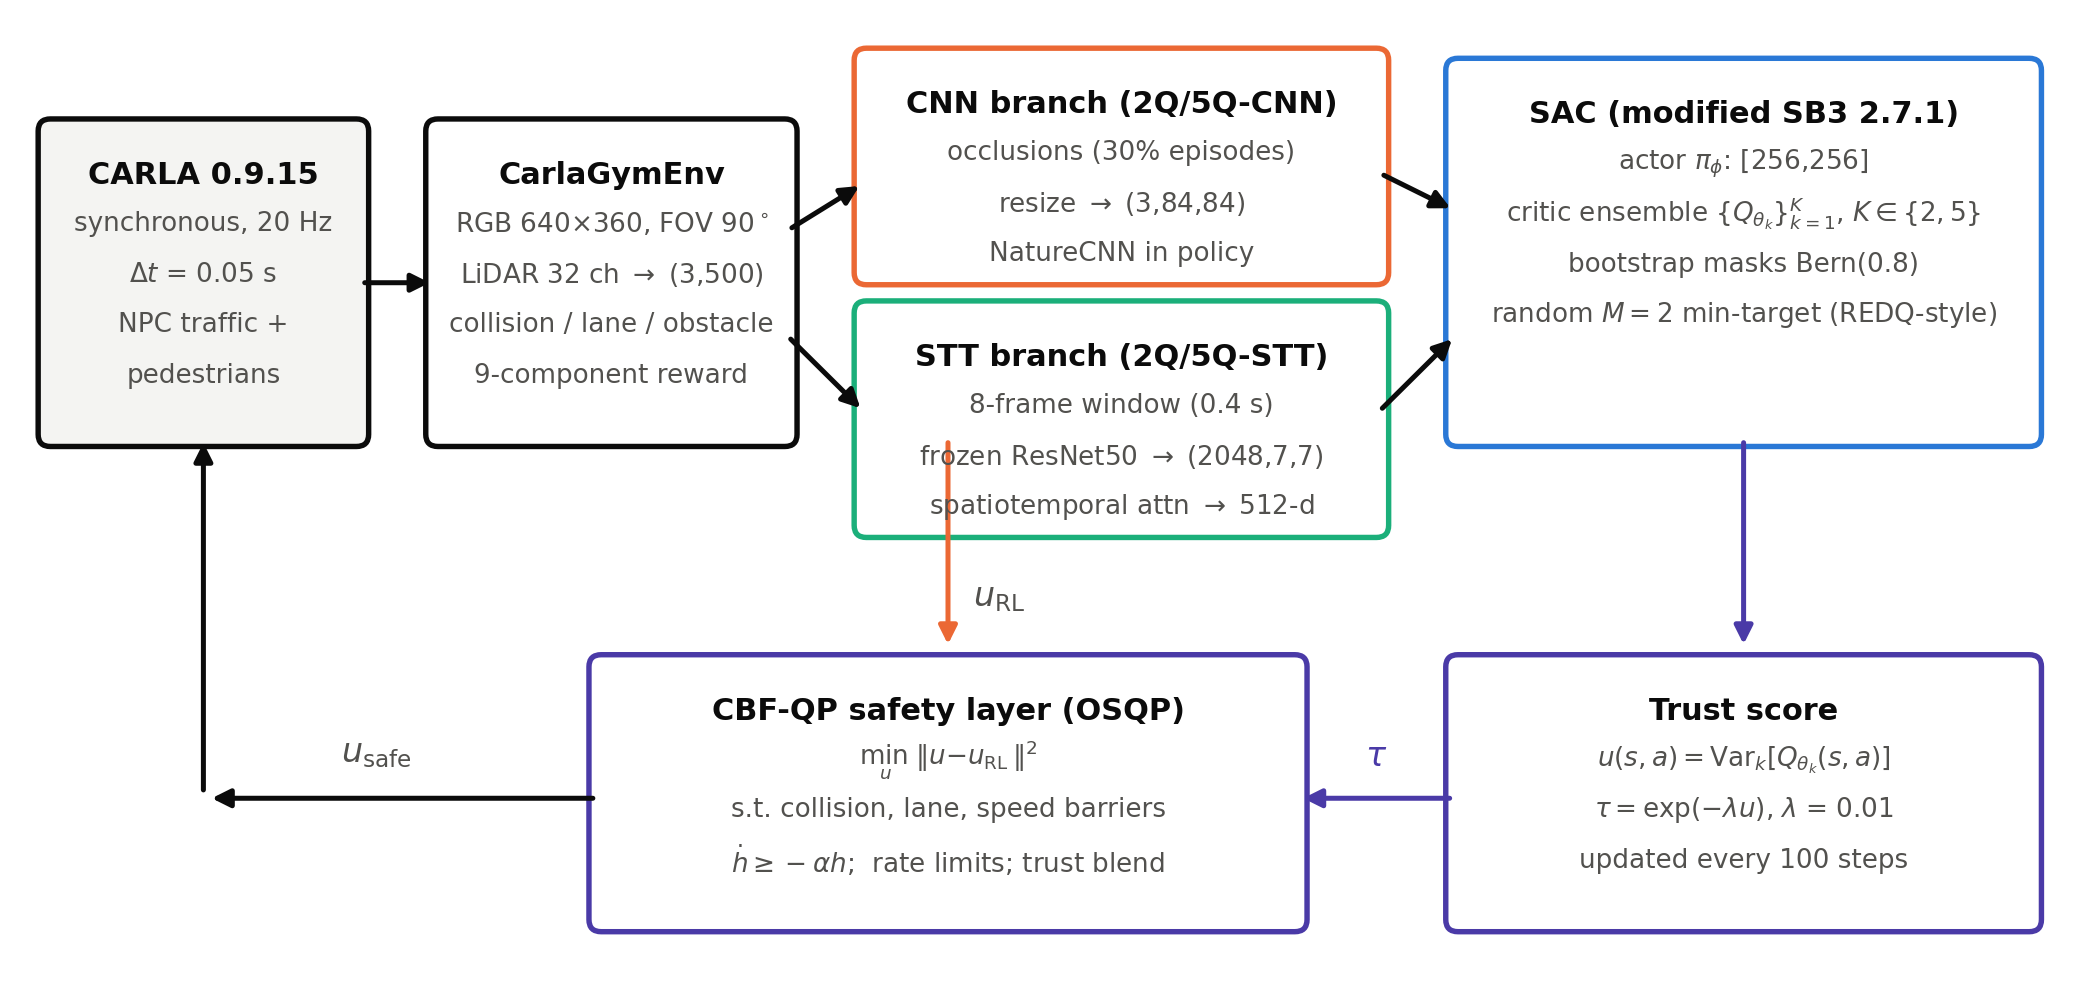
\includegraphics[width=0.95\textwidth]{Assets/system_architecture.png}
    \caption{System architecture. CARLA runs synchronously at 20 Hz. Observations flow through one of two perception branches into a SAC agent whose critic is a $K$-member bootstrapped ensemble. The ensemble's variance at the policy action is mapped to a trust score $\tau$ that modulates the CBF-QP safety layer, which minimally corrects the policy action before it is applied to the vehicle.}
    \label{fig:arch}
\end{figure*}

Fig.~\ref{fig:arch} shows the complete control loop. A custom Gym environment wraps the CARLA client and exposes camera, LiDAR, and event sensors. Depending on the variant, the observation is either a downsampled image consumed by a convolutional policy, or a 512-dimensional embedding produced by a spatiotemporal transformer pipeline. The SAC agent proposes an action $u_{\mathrm{RL}} = [\text{steer}, \text{throttle}, \text{brake}]$. Before execution, a CBF-QP layer projects $u_{\mathrm{RL}}$ onto the safe set defined by collision, lane, and speed barriers; the projection's tightness is modulated by the trust score computed from the critic ensemble. The executed safe action $u_{\mathrm{safe}}$ drives the simulator, and a small penalty proportional to the correction magnitude is added to the reward so the policy is nudged to internalize the safe behavior.

\section{Methodology}

\subsection{Simulation Environment and Driving Task}
All experiments run in CARLA 0.9.15 in synchronous mode at a fixed timestep of $\Delta t = 0.05$\,s (20\,Hz), with the traffic manager synchronized to the world clock so that non-player vehicles tick on the same schedule as the ego vehicle---a detail that eliminates phantom collisions caused by asynchronous actor updates. Up to 200 NPC vehicles (capped by the map's spawn capacity) and up to 200 pedestrians with randomized walking speeds of 0.5--1.5\,m/s populate the town, creating dense, stochastic traffic.

The ego vehicle carries a front RGB camera ($640{\times}360$, $90^{\circ}$ FOV), a 32-channel LiDAR (50\,m range, subsampled to a fixed 500 points), and collision, lane-invasion, and obstacle-detection sensors. Each episode teleports the ego to a randomly selected spawn point with at least 10\,m clearance to the nearest vehicle, then generates a 40-waypoint route at 5\,m spacing ($\approx$195\,m) along the road ahead. The agent must make progress along this route while staying in lane, respecting the speed limit queried dynamically from the map, and avoiding collisions. Episodes terminate on collision, on reaching the route endpoint, after 1{,}000 steps (50\,s), or if the vehicle remains essentially stationary on a clear road.

The action space is $[\text{steer}, \text{throttle}, \text{brake}] \in [-1,1] \times [0,1] \times [0,1]$. Placing the pedals on $[0,1]$ rather than $[-1,1]$ is deliberate: a freshly initialized SAC policy outputs actions near the center of the box, which under a symmetric range would mean zero throttle and a vehicle that never moves. The step function additionally enforces throttle/brake mutual exclusion with a small deadzone, matching how a human driver uses one pedal at a time.

\subsection{Perception Pipelines}
\subsubsection{CNN variants (2Q-CNN, 5Q-CNN)}
The image observation is resized to $3{\times}84{\times}84$ and consumed by SAC's convolutional policy (the standard three-layer Nature-CNN feature extractor followed by $[256,256]$ fully connected heads). This branch is trained fully end-to-end: perception and control gradients flow together, and the compact input keeps the replay buffer memory-efficient.

\subsubsection{Spatiotemporal transformer variants (2Q-STT, 5Q-STT)}
The STT branch targets temporal reasoning: closing speeds, relative motion, and dynamics that a single frame cannot show. A ResNet50 trunk \cite{he2016resnet}, initialized from ImageNet weights \cite{deng2009imagenet} and kept frozen, maps each frame to a $2048{\times}7{\times}7$ feature map. An 8-frame sliding window (0.4\,s of history at 20\,Hz) of such maps enters a spatiotemporal encoder that applies factorized (divided) space-time attention in the style of \cite{vaswani2017attention}: each of four blocks attends over the 8 temporal positions of every spatial patch, then over the 49 spatial patches of every frame, with learned spatial and temporal positional embeddings. A stack of five further transformer blocks fuses the temporal embedding with a projection of the current frame's pooled features, producing a single 512-dimensional embedding per step. The SAC policy for these variants is a multilayer perceptron over this embedding.

A practical design decision is that the perception pipeline runs \emph{inside the observation wrapper}, upstream of the RL algorithm. The replay buffer therefore stores 512-float embeddings (2\,KB) instead of raw frames ($\approx$690\,KB), a $\sim$340$\times$ memory reduction that allows a 50{,}000-transition buffer to fit comfortably in RAM. The encoder can be initialized from a pretrained checkpoint via \texttt{--encoder-path}, and the training scripts snapshot the encoder weights alongside every SAC checkpoint.

\subsection{SAC with a Bootstrapped Critic Ensemble}
\label{sec:sb3}
We vendor Stable-Baselines3 2.7.1 \cite{raffin2021sb3} and modify its SAC implementation \cite{haarnoja2018sac}. The stock twin critic is replaced by an \texttt{EnsembleCritic} holding $K$ independent Q-networks $\{Q_{\theta_k}\}_{k=1}^{K}$, $K \in \{2, 5\}$ in our experiments. Three mechanisms keep the ensemble's disagreement informative:

\textbf{Bootstrap masking.} At every training step, a Bernoulli($0.8$) mask over (sample, critic) pairs determines which transitions each critic learns from, so each critic sees a different $\sim$80\% subsample of every minibatch. Without this, all critics would fit identical targets on identical data and their variance would collapse; with it, ensemble variance behaves like a bootstrapped epistemic estimate \cite{lakshminarayanan2017ensembles}.

\textbf{Randomized subset target.} The temporal-difference target uses a REDQ-style random subset \cite{chen2021redq}: at each update, $M{=}2$ of the $K$ target critics are sampled and the target is
\begin{equation}
y = r + \gamma \Big( \min_{k \in \mathcal{M}, |\mathcal{M}|=2} Q_{\bar\theta_k}(s', a') - \alpha_{\mathrm{ent}} \log \pi(a'|s') \Big),
\end{equation}
so target pessimism does not grow with $K$ and the $K{=}2$ configuration recovers standard clipped double-Q \cite{fujimoto2018td3}. The critic loss averages the masked per-critic mean-squared errors; the actor maximizes the minimum over all $K$ critics with SAC's automatic entropy temperature (target entropy $-3$ for the 3-D action space).

\subsection{Trust Score from Ensemble Uncertainty}
The modified critic exposes, for any state-action pair,
\begin{equation}
u(s,a) = \operatorname{Var}_{k}\!\big[Q_{\theta_k}(s,a)\big], \qquad
\tau(s,a) = \exp\!\big(-\lambda\, u(s,a)\big),
\label{eq:trust}
\end{equation}
with $\lambda = 0.01$. During training, a callback evaluates \eqref{eq:trust} every 100 environment steps at the deterministic policy action for the current observation and pushes the resulting $\tau \in [0,1]$ into the safety layer. High critic agreement ($u \to 0$) yields $\tau \to 1$ and the policy is trusted; high disagreement drives $\tau$ toward 0 and the safety layer becomes more conservative. Both $u$ and $\tau$ are logged to TensorBoard throughout training, which is what allows Section~\ref{sec:results} to verify that the signal actually discriminates in practice.

\subsection{CBF-QP Safety Layer}
The safety layer solves, at every control step, the minimally invasive projection
\begin{equation}
u_{\mathrm{safe}} = \arg\min_{u}\ \tfrac{1}{2}\left\lVert u - u_{\mathrm{RL}} \right\rVert^2
\quad \text{s.t.} \quad A(x)\, u \geq -\,\boldsymbol{\alpha} \circ h(x),
\label{eq:qp}
\end{equation}
a discrete-time CBF condition $\dot h \geq -\alpha h$ \cite{ames2017cbf} over three barriers built from the environment state $x = \{d_{\mathrm{col}}, y_{\mathrm{lane}}, v, v_{\mathrm{limit}}\}$:
\begin{align}
h_{\mathrm{col}} &= d_{\mathrm{col}} - d_{\min}, & d_{\min} &= 1.2\,\mathrm{m},\\
h_{\mathrm{lane}} &= y_{\max} - |\hat y_{\mathrm{lane}}|, & y_{\max} &= 1.9\,\mathrm{m},\\
h_{\mathrm{speed}} &= v_{\mathrm{limit}} - v, &&
\end{align}
with $\alpha_{\mathrm{col}} = \alpha_{\mathrm{speed}} = 1.0$ and a deliberately softer $\alpha_{\mathrm{lane}} = 0.8$ so the lane barrier guides rather than fights the policy through curves. Three refinements matter in practice:

\textbf{Speed-dependent control authority.} The Lie-derivative rows scale with $v / v_{\mathrm{nom}}$ ($v_{\mathrm{nom}} = 10$\,m/s), with braking authority saturating at high speed---capturing that pedals move the safety margins more when the car is faster.

\textbf{Proactive lane keeping.} The lane barrier uses a one-step-ahead offset prediction $\hat y = y + \dot\psi\, \Delta t$ from a kinematic bicycle model (wheelbase 2.7\,m), so the constraint acts before the vehicle drifts out rather than after.

\textbf{Rate limiting and trust blending.} The QP solution is rate-limited (steering change $\leq 0.5$/step, net pedal change $\leq 1.9$/step) to avoid actuator chatter, and then blended toward a conservative fallback action in proportion to distrust:
\begin{equation}
u_{\mathrm{final}} = \big(1 - 0.3(1-\tau)\big)\, u_{\mathrm{safe}} + 0.3 (1-\tau)\, u_{\mathrm{fb}},
\label{eq:blend}
\end{equation}
so that even at zero trust, at most 30\% of the fallback is mixed in and the learned policy is never fully overridden. The QP is solved with OSQP \cite{stellato2020osqp} with polishing enabled; a solver failure falls back to the previous safe action. Finally, the wrapper subtracts a penalty of $0.003 \cdot \lVert u_{\mathrm{safe}} - u_{\mathrm{RL}} \rVert$ from the reward whenever the correction is non-negligible, giving the policy a gentle incentive to propose actions that already satisfy the barriers.

\subsection{Reward Design}
The reward sums nine weighted dense components with event and terminal terms (Table~\ref{tab:reward}). The dense terms are dominated by forward progress---\emph{movement} (weight 8) and \emph{waypoint progress} (weight 4, including a $+12$ milestone per waypoint crossed)---so the gradient consistently favors driving over standing still, while graded penalties for lane offset, tailgating (a time-to-collision band computed from forward LiDAR returns), encroaching the opposite lane, and closing on obstacles shape \emph{how} the agent drives. A constant alive bonus guarantees survival is never worth less than termination, and a capped stalling penalty with a 3-second grace window discourages the degenerate stop-forever policy without punishing legitimate waiting in traffic. Collisions terminate the episode at $-600$; completing the route pays $+240$ plus a time bonus of up to $+120$. A stuck episode (planar speed below 1\,m/s after step 200) terminates with an additional $-50$, and the safety-layer wrapper subtracts $0.003\,\lVert u_{\mathrm{safe}}-u_{\mathrm{RL}}\rVert$ whenever its correction is non-negligible.

\textbf{Provenance.} All reported runs were trained from branch \texttt{testing} of the public repository, whose \texttt{\_compute\_reward()} is the weighted-sum form of Table~\ref{tab:reward}; the function is byte-identical at every commit spanning the training window, so every variant optimized the same objective. The repository's default \texttt{main} branch (last updated 2026-04-21) still carries an earlier five-term reward (collision $-25$, speed zones, small infraction penalties, $+3$ per waypoint, $+300$ on completion) in which the shaping methods above are present but not invoked; it was not used for any result in this paper. The repository additionally vendors the third-party CARLA-GymDrive framework \cite{morgado2024gymdrive}, whose own ten-term reward (collision, steering and pedal jerk, speed, zero-speed, opposite-lane, CBF-correction, traffic-light, destination, and waypoint terms) is not imported by any experiment, environment, wrapper, or callback.

\begin{table*}[htbp]
\centering
\caption{Reward function exactly as implemented in \texttt{CarlaGymEnv.\_compute\_reward()} (\texttt{tests/pipeline\_carla\_test.py}, branch \texttt{testing}, commit \texttt{85e5658}). Line numbers refer to that file. The function is byte-identical at commits \texttt{e045625} (2026-05-15), \texttt{bd92adc} (2026-06-06), and \texttt{85e5658} (2026-06-22), which bracket the entire training window. $v_f$: forward speed; $v_\perp$: lateral speed; $v_{\lim}$: map speed limit; $y$: lane offset; $\delta$: steering; $\rho$: waypoint completion ratio; $n_{\text{stall}}$: consecutive stalled steps.}
\label{tab:reward}
\small
\begin{tabular}{@{}llrl@{}}
\toprule
\textbf{Term} & \textbf{Line} & \textbf{Weight} & \textbf{Range / definition} \\
\midrule
\multicolumn{4}{@{}l}{\emph{Dense components (summed after weighting)}} \\
alive              & 1119 & ---   & $+0.5$ constant \\
movement           & 1120 & $8.0$ & $\approx[-1.6,+19.2]$; $15\,\mathrm{clip}(v_f/v_{\lim},0,1.2)+1.5\,a_{\text{align}}-0.9\min(v_\perp,4)+\text{move}$ \\
safe\_following    & 1124 & $4.5$ & $[-8.0,+0.7]$ piecewise in time-to-collision from forward LiDAR returns \\
waypoint\_progress & 1122 & $4.0$ & $[-7,+23]$; $3.5\,\mathrm{clip}(\Delta d,\pm2)+12\cdot\mathbb{1}[\text{waypoint crossed}]+4\rho$ \\
lane\_centering    & 1121 & $3.5$ & $[-5.0,+0.8]$ piecewise in $|y|$, minus $0.5|\delta|\min(v/5,1)$ \\
obstacle\_avoidance& 1128 & $3.0$ & $[-17.5,0]$ piecewise in detected-obstacle range \\
safety\_buffer     & 1126 & $2.5$ & $[-8.8,+0.15]$ in collision distance ($+0.15$ when the CBF prevented a collision) \\
containment        & 1127 & $2.5$ & $[-7.0,0]$ for $|y|>1.75$\,m (opposite-lane encroachment) \\
traffic\_flow      & 1123 & $1.0$ & $\approx[-2.1,+11.8]$ speed band $+$ clear-road nudge $-$ jerk $-$ hard braking \\
yielding           & 1125 & $0.4$ & $\{-0.7,-0.15,0,+0.2\}$ rear-traffic etiquette \\
\midrule
\multicolumn{4}{@{}l}{\emph{Event terms (added to the same sum when triggered)}} \\
lane\_invasion     & 1131 & --- & $-15.0$ on a lane-invasion sensor event \\
close\_obstacle    & 1134 & --- & $-6.0$ if an obstacle is detected within 8\,m \\
speeding           & 1137 & --- & $-8.0\,(v/v_{\lim}-1.08)$ if $v>1.08\,v_{\lim}$ \\
stalling           & 1144 & --- & $-\min(3.0,\,0.3+0.05\,n_{\text{stall}})$, armed after step 60 on a clear road \\
\midrule
\multicolumn{4}{@{}l}{\emph{Terminal and wrapper terms}} \\
collision          & 1089 & --- & step reward is exactly $-600$ (early return; dense terms suppressed); episode ends \\
completion         & 1147 & --- & $240+120\,\mathrm{clip}(1-t/T,0,1)\in[240,360]$, $T{=}1000$; summed with dense terms; episode ends \\
stuck              & 1350 & --- & $-50$ if planar speed $<1$\,m/s after step 200 (applied in \texttt{step()}); episode ends \\
CBF correction     & 1732 & --- & $-0.003\,\lVert u_{\mathrm{safe}}-u_{\mathrm{RL}}\rVert$ if $\lVert\Delta u\rVert>0.01$ (safety-layer wrapper) \\
\bottomrule
\end{tabular}
\end{table*}

\subsection{Aleatoric Uncertainty via Sensor Occlusion}
Because the policy drives primarily from one camera, we train under explicit aleatoric degradation of that sensor \cite{kendall2017uncertainties}. In 30\% of episodes (sampled at reset and held for the episode, mimicking a persistent physical cause such as a fouled lens or blocked mount), the image-space observation pipeline applies: (i) opaque black bars of 20--99\,px at the top, bottom, or both edges of the $360$-row frame (up to $\sim$55\% of image height); (ii) a saturated noise band---$\mathcal{N}(200, 30)$ clipped to $[0,255]$, resampled every step---covering one third of the image width at the left, center, or right, emulating glare or blown exposure; and (iii) random LiDAR point dropout retaining 60\% of returns. The CNN variants train directly on these degraded frames, so robustness to partial blindness is baked into the learned representation rather than patched on afterward.

\section{Experimental Setup}
\begin{table}[htbp]
\centering
\caption{The Four Trained Variants}
\label{tab:variants}
\begin{tabular}{lcccc}
\toprule
 & \textbf{2Q-CNN} & \textbf{5Q-CNN} & \textbf{2Q-STT} & \textbf{5Q-STT} \\
\midrule
Critics $K$ & 2 & 5 & 2 & 5 \\
Policy input & $84^2$ img & $84^2$ img & 512-d emb & 512-d emb \\
Feature extractor & CNN (e2e) & CNN (e2e) & STT & STT \\
Occlusion training & yes & yes & --- & --- \\
Steps trained & 1{,}000k & 784k & 880k & 150k \\
Telemetry span & 10--390k & 0--784k & 0--221k, & 90--153k \\
 & & (full) & 870--884k & \\
\bottomrule
\end{tabular}
\end{table}

\begin{table}[htbp]
\centering
\caption{SAC and Safety-Layer Hyperparameters (all variants)}
\label{tab:hyper}
\begin{tabular}{ll}
\toprule
Learning rate & $3\times10^{-4}$ (Adam) \\
Batch size / buffer size & 64 / 50{,}000 \\
Discount $\gamma$ / soft update $\tau_{\mathrm{polyak}}$ & 0.99 / 0.005 \\
Train freq / gradient steps & 1 / 1 \\
Entropy coefficient & auto (target $-3$) \\
Actor / critic networks & $[256, 256]$ \\
Bootstrap mask rate & Bernoulli(0.8) \\
Target subset size $M$ & 2 \\
Trust decay $\lambda$ & 0.01 \\
Trust update period & 100 steps \\
CBF $(\alpha, \alpha_{\mathrm{lane}}, d_{\min}, y_{\max})$ & $(1.0,\, 0.8,\, 1.2\,\mathrm{m},\, 1.9\,\mathrm{m})$ \\
Correction penalty & $0.003 \cdot \lVert \Delta u \rVert$ \\
Checkpoint period & 10{,}000 steps (+ replay buffer) \\
\bottomrule
\end{tabular}
\end{table}

Table~\ref{tab:variants} summarizes the four variants and Table~\ref{tab:hyper} the shared hyperparameters. Training was distributed over two machines---a dedicated GPU server for the early phases and a Windows workstation for the later ones---with CARLA always running as a separate server process. Every experiment script supports \texttt{--load-checkpoint} resumption: model weights, optimizer state, the step counter, and (where saved) the replay buffer are restored, so a run can migrate between machines and continue without resetting its step counter. The 5Q-CNN variant exercises this end to end: it trained from initialization to $\sim$566k steps on the GPU server, was resumed on the workstation from its 560k checkpoint, and continued to 784k, yielding the single continuous learning curve reported below. Training telemetry is logged per step---episode statistics, per-episode safety summaries (collision, lane-invasion, and CBF-intervention rates), and the live trust score and ensemble variance.

Wall-clock throughput differed sharply by perception design, and we report it because it shaped the training budgets in Table~\ref{tab:variants}: the CNN variants sustained roughly 3--6 environment steps per second, while the 5Q-STT variant---which pushes eight ResNet50 forward passes plus the full attention stack through the GPU at every environment step, on top of the five-critic SAC update---ran at approximately \emph{one iteration per second}. Despite that cost we carried 5Q-STT past 90{,}000 steps (150{,}000 at its final checkpoint), enough to observe its learning dynamics, though not to parity with its siblings.

\section{Results}
\label{sec:results}

\subsection{Training Performance}
\begin{figure*}[htbp]
    \centering
    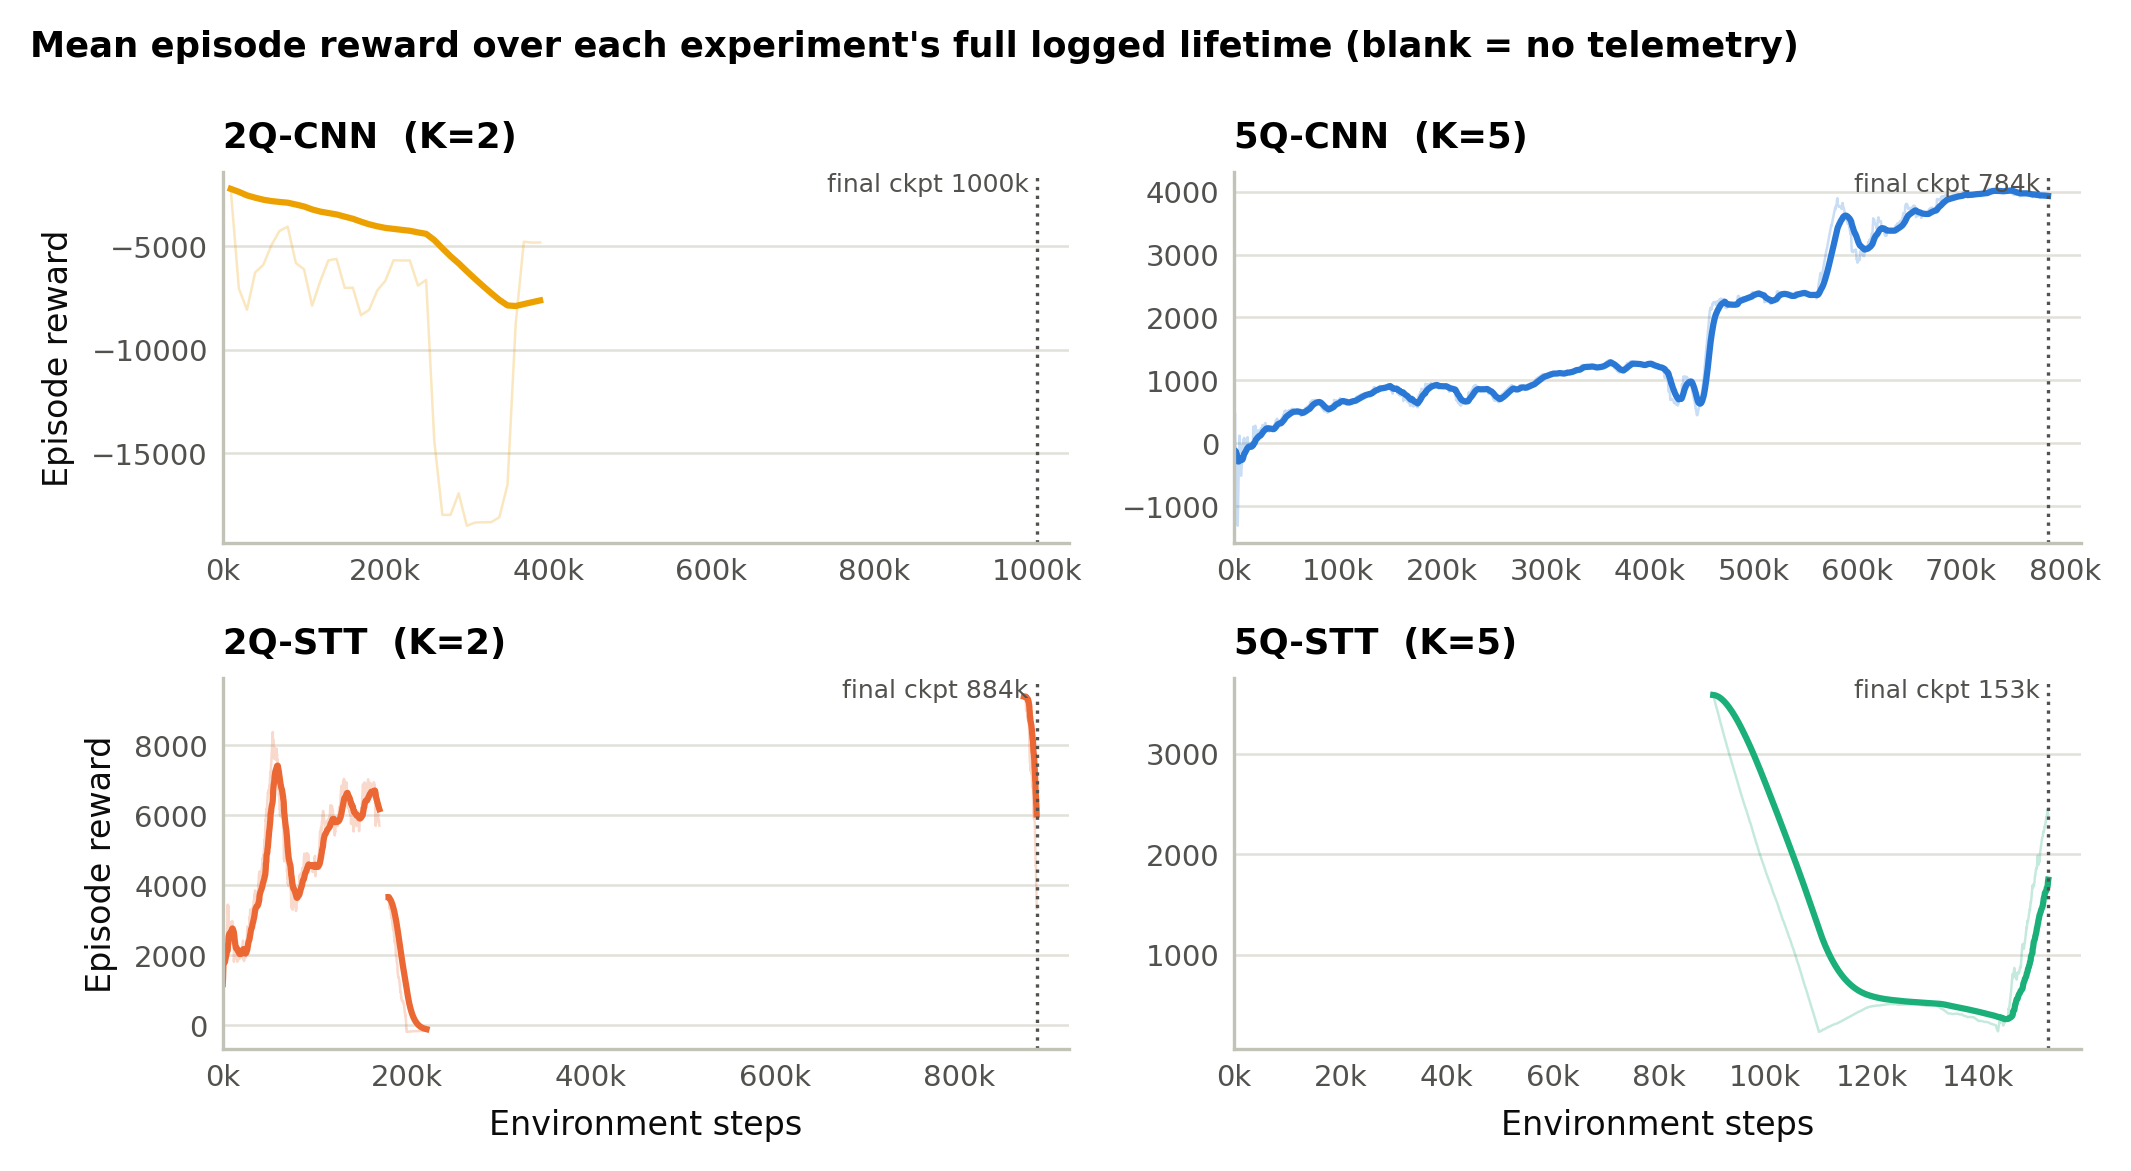
\includegraphics[width=0.98\textwidth]{Assets/full_runs_overview.png}
    \caption{Mean episode reward for every experiment over its complete logged lifetime, from step zero to the final checkpoint (dotted line). Only real telemetry is drawn; blank spans are windows with no event files (2Q-CNN 390k--1M, 2Q-STT 221k--870k, 5Q-STT before 90k). Faint lines are raw values; bold lines are exponentially smoothed. Per-experiment multi-panel versions of these curves (reward, episode length, trust, ensemble variance, CBF rate) accompany the released telemetry.}
    \label{fig:overview}
\end{figure*}

\begin{figure}[htbp]
    \centering
    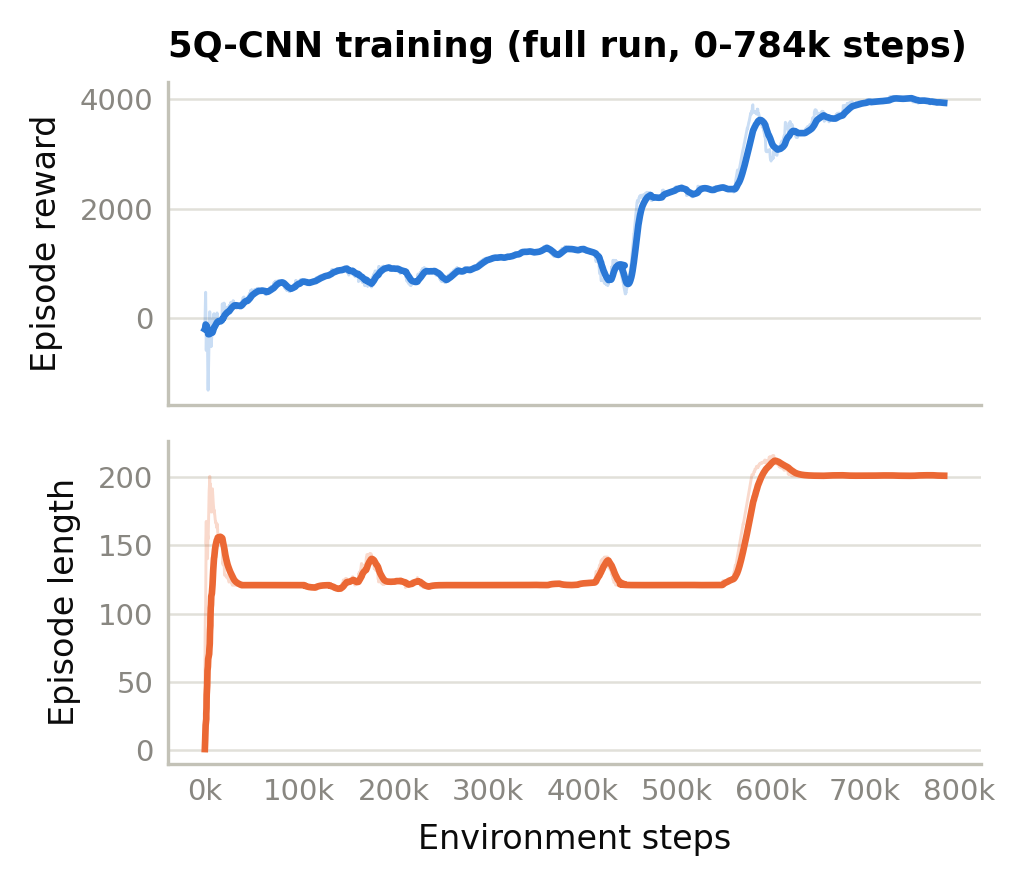
\includegraphics[width=0.95\linewidth]{Assets/5qcnn_training.png}
    \caption{5Q-CNN training telemetry over the complete run (0--784k steps, spanning both machines): mean episode reward (top) and mean episode length (bottom). Faint lines are raw values; bold lines are exponentially smoothed.}
    \label{fig:5qcnn}
\end{figure}

\begin{figure}[htbp]
    \centering
    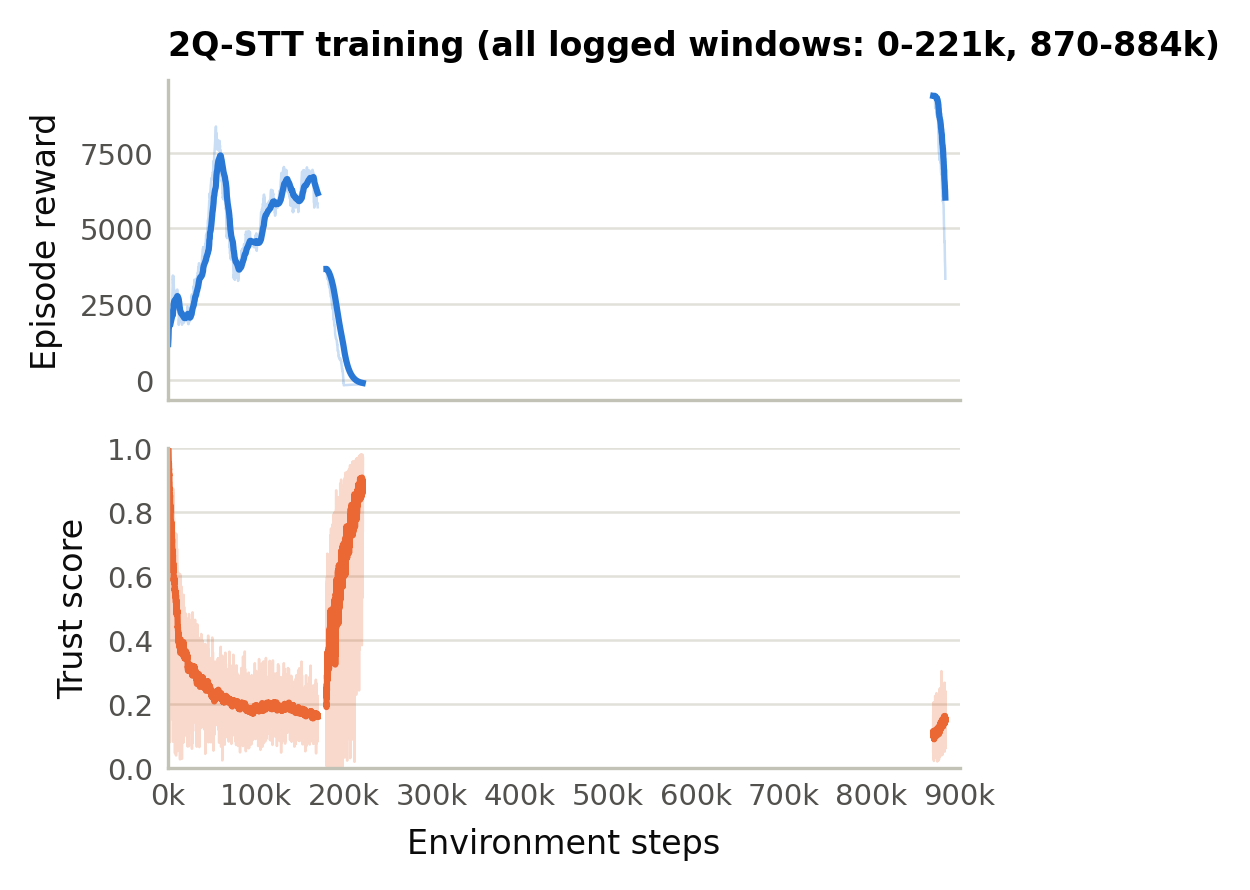
\includegraphics[width=0.95\linewidth]{Assets/2qstt_training.png}
    \caption{2Q-STT telemetry for the two logged windows---early training (0--170k) and late training (870k--884k): mean episode reward (top) and live trust score (bottom). Trust declines as the two-critic ensemble's disagreement grows with the value scale.}
    \label{fig:2qstt}
\end{figure}

\begin{figure}[htbp]
    \centering
    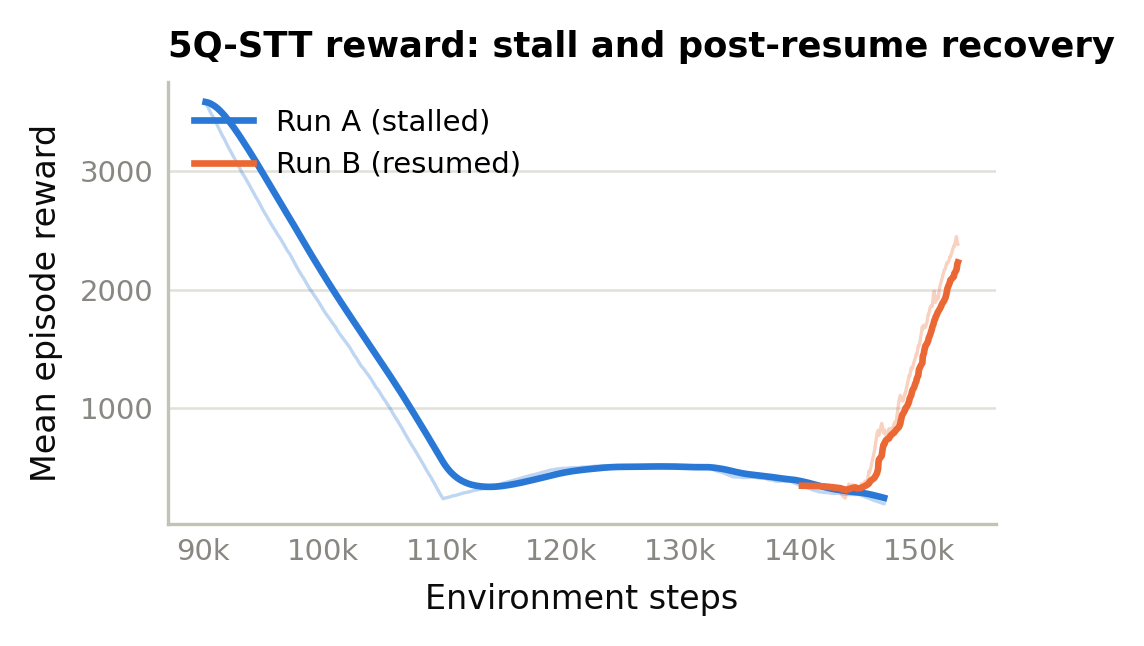
\includegraphics[width=0.95\linewidth]{Assets/5qstt_runs.png}
    \caption{5Q-STT mean episode reward across its two training sessions. After a mid-training slump, resuming from the 140k checkpoint (with restored replay buffer) produced a rapid recovery.}
    \label{fig:5qstt}
\end{figure}

\begin{figure}[htbp]
    \centering
    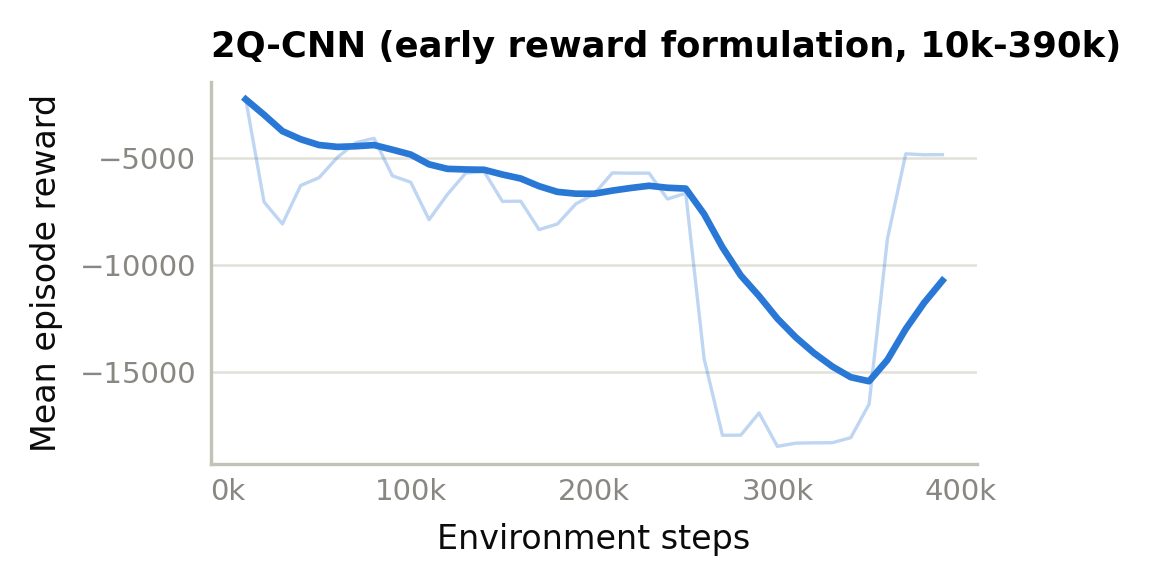
\includegraphics[width=0.95\linewidth]{Assets/2qcnn_training.png}
    \caption{2Q-CNN mean episode reward over its logged segment (10k--390k steps). This earliest run used a previous, sparser reward formulation, so its absolute scale is not comparable to the later variants.}
    \label{fig:2qcnn}
\end{figure}

Fig.~\ref{fig:overview} places all four experiments on a common footing, each drawn from step zero to its final checkpoint with logging gaps left blank. Fig.~\ref{fig:5qcnn} shows the best-instrumented variant, 5Q-CNN, across its complete 784k-step lifetime. Mean episode reward rises monotonically in the large from $-200$ at initialization (with an early trough of $-1{,}312$ as the untrained policy collides and stalls) through $\approx$1{,}500 by 400k steps, then accelerates through a second learning phase to a peak of 4{,}046, closing at 3{,}924. The episode-length trace shows the corresponding behavioral shift: episodes stabilize near 121 steps for most of training and then lengthen to $\approx$201 after 560k steps as the agent sustains longer collision-free drives. This is the full arc of a safety-shielded agent learning to drive from scratch, and it is the paper's primary training result.

The 2Q-STT variant (Fig.~\ref{fig:2qstt}) learns quickly in its early window, with mean episode reward rising from 1{,}175 to a peak of 8{,}377 within 170k steps, and it crossed up to 62.5\% of its route waypoints in single episodes. Its trust trace is equally informative and is discussed in Section~\ref{sec:trustres}. The 5Q-STT run (Fig.~\ref{fig:5qstt}) illustrates the value of the checkpoint-resume machinery: after a mid-training slump, resuming from the 140k checkpoint recovered mean episode reward from $\approx$300 to $\approx$2{,}384 within 13k steps. Fig.~\ref{fig:2qcnn} shows the earliest 2Q-CNN run under the project's initial reward formulation; the reward function was substantially redesigned afterward (Table~\ref{tab:reward}), and the later variants' healthier curves reflect that redesign.

\subsection{The Trust Mechanism Is Live and Discriminating}
\label{sec:trustres}
\begin{figure}[htbp]
    \centering
    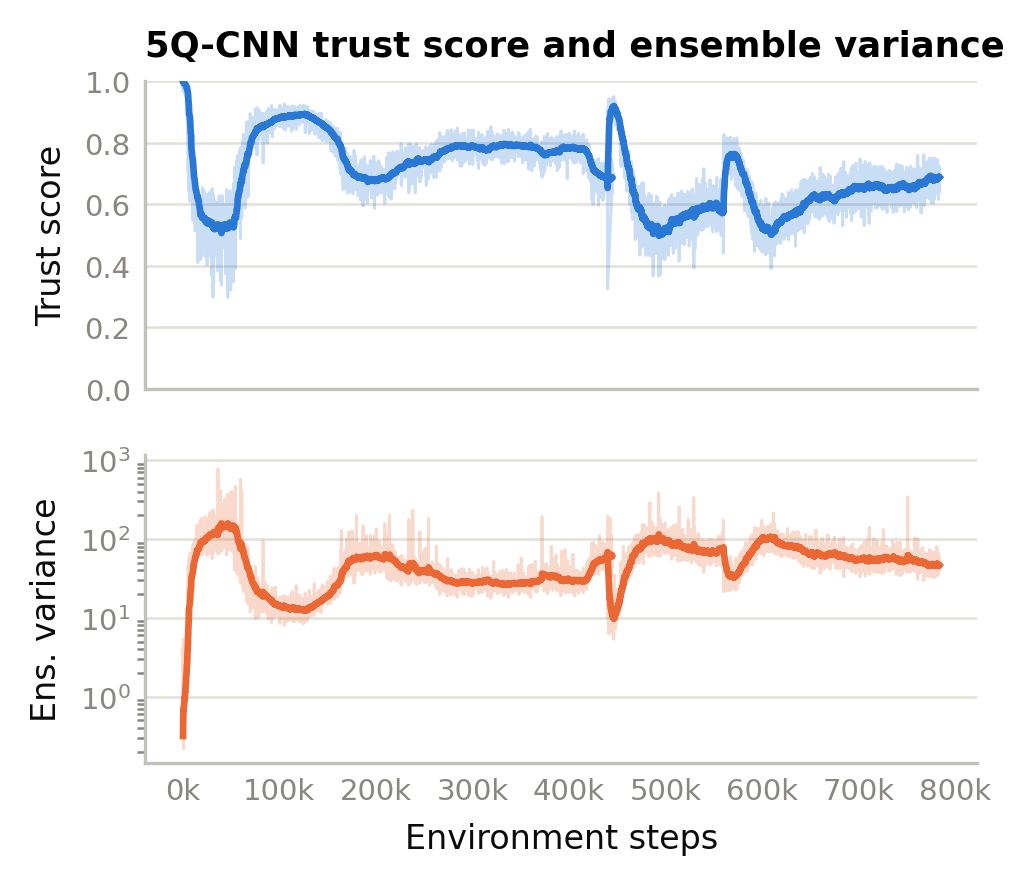
\includegraphics[width=0.95\linewidth]{Assets/5qcnn_trust.png}
    \caption{5Q-CNN live trust score (top) and critic-ensemble variance, log scale (bottom). The trust score moves across a wide dynamic range as the ensemble's disagreement evolves---the modulation signal neither saturates at 1 (which would disable the mechanism) nor pins at 0 (which would freeze the policy out).}
    \label{fig:trust}
\end{figure}

A design risk identified before training was that the trust signal could be degenerate---saturated at $\tau \approx 1$ (making modulation a no-op) or collapsed at $\tau \approx 0$ (permanently maximal intervention). The full-lifetime telemetry rules this out (Fig.~\ref{fig:trust}). Over 5Q-CNN's complete 784k-step run, trust spans $0.297$--$0.998$ and ends near $0.70$, tracking inverse ensemble variance as designed and traversing the informative middle of its range for essentially the whole run rather than pinning at either bound. The trace is legible as a record of the learner's own competence: trust starts near 1.0 while the freshly initialized critics trivially agree, drops sharply to $\approx$0.5 during the first 50k steps as the ensemble confronts the reward landscape and disagrees, recovers to $\approx$0.85 as value estimates consolidate, and thereafter oscillates in a $0.5$--$0.8$ band, dipping at each resume boundary---exactly where a newly reloaded critic should be least certain---before climbing again.

The comparison across variants is equally clean. On 2Q-STT (Fig.~\ref{fig:2qstt}, bottom), trust decays from 1.0 to $\approx$0.17 over the first 170k steps and remains near $0.09$--$0.30$ at 880k, because its two-critic variance grows with the value scale; on 5Q-STT's recovered session it holds at $0.61$--$0.997$. Each learner is therefore held to a different degree of constraint, determined by its own measured uncertainty rather than by a hand-set schedule---which is precisely the behavior the mechanism was designed to produce.

\subsection{Five Critics Estimate Uncertainty Better Than Two}
\begin{figure}[htbp]
    \centering
    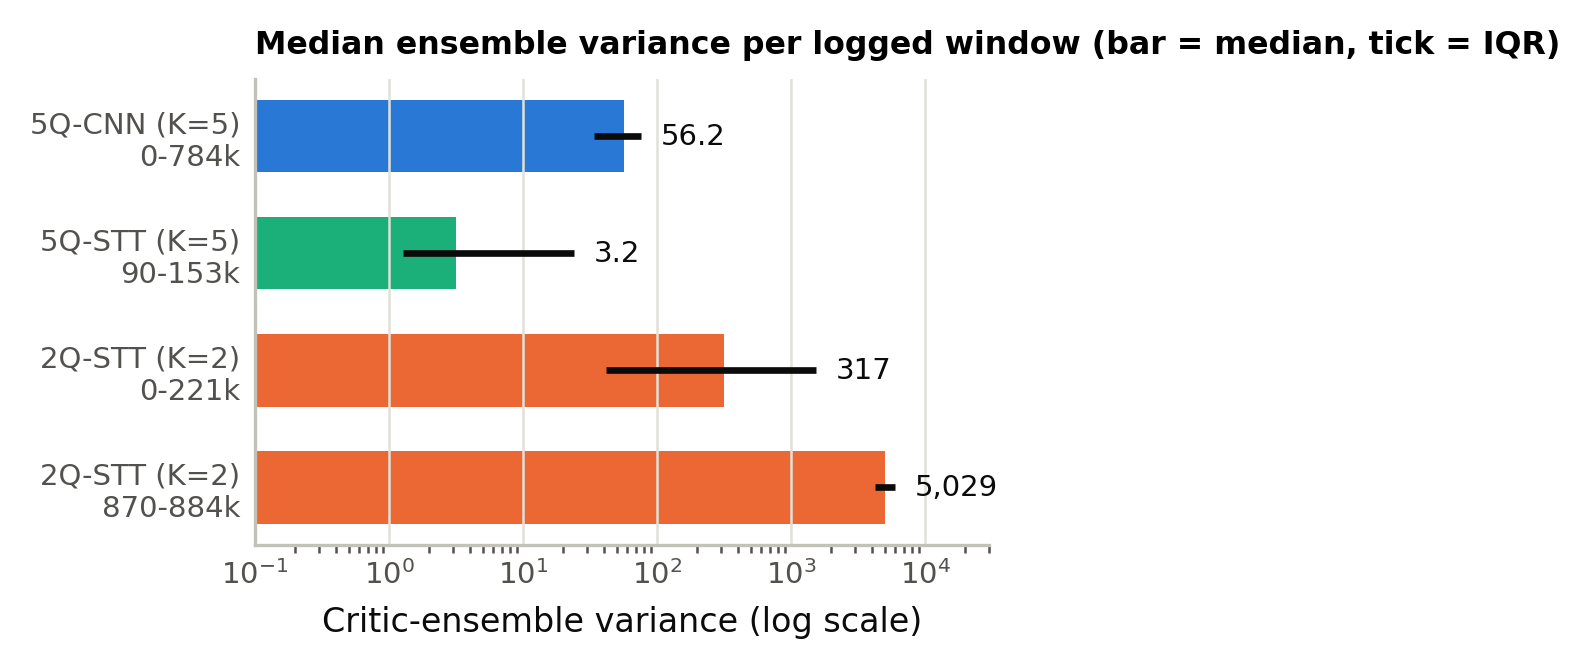
\includegraphics[width=0.95\linewidth]{Assets/uncertainty_compare.png}
    \caption{Critic-ensemble variance per logged window (bar = median, black tick = interquartile range, log scale). The two $K{=}5$ ensembles sit one to two orders of magnitude below the $K{=}2$ ensemble, and the $K{=}2$ gap widens rather than closes with further training (0--221k versus 870--884k).}
    \label{fig:uncertainty}
\end{figure}

Fig.~\ref{fig:uncertainty} summarizes ensemble variance per logged window. The medians tell the story compactly: $56$ for 5Q-CNN over its full 784k steps and $3.2$ for 5Q-STT, against $317$ for 2Q-STT in its first 221k steps and $5{,}029$ in its final window---and the interquartile ranges of the two ensemble sizes do not overlap. The recovered early-training telemetry also makes a \emph{step-matched} comparison possible rather than merely a suggestive one. Over the identical window 0--170k steps, the $K{=}5$ ensemble holds its variance in the $10$--$10^2$ band and \emph{decreases} after an initial exploratory peak, while the $K{=}2$ ensemble rises monotonically past $10^3$ and reaches $\approx$2{,}500 by 170k---one to two orders of magnitude higher on an equal training budget. The gap widens rather than closes with further training: at 880k steps the two-critic ensemble sits at $\approx$3{,}700 (peaking near $2.4\times10^4$), whereas the five-critic ensembles remain between $1$ and $10^2$.

Critic-loss convergence corroborates the reading: 5Q-CNN's critic loss descends to $\approx$615, whereas 2Q-STT's remains at $\approx$27{,}600 and does not converge over its logged segment. This is consistent with the statistics of the estimator itself---a two-sample variance is a one-degree-of-freedom estimate with very large spread---and with REDQ's finding that larger randomized ensembles stabilize value learning \cite{chen2021redq}. Because our trust score is an exponential function of this variance \eqref{eq:trust}, a noisy two-sample estimate does not merely add noise: it biases the safety layer toward permanent distrust, which is what the 2Q-STT trust trace shows. For a trust signal that gates a safety system, the practical recommendation is unambiguous---use the larger ensemble; the cost of three additional critic heads is negligible beside CARLA simulation itself.

\subsection{Safety-Layer Engagement and Collision Outcomes}
\begin{figure}[htbp]
    \centering
    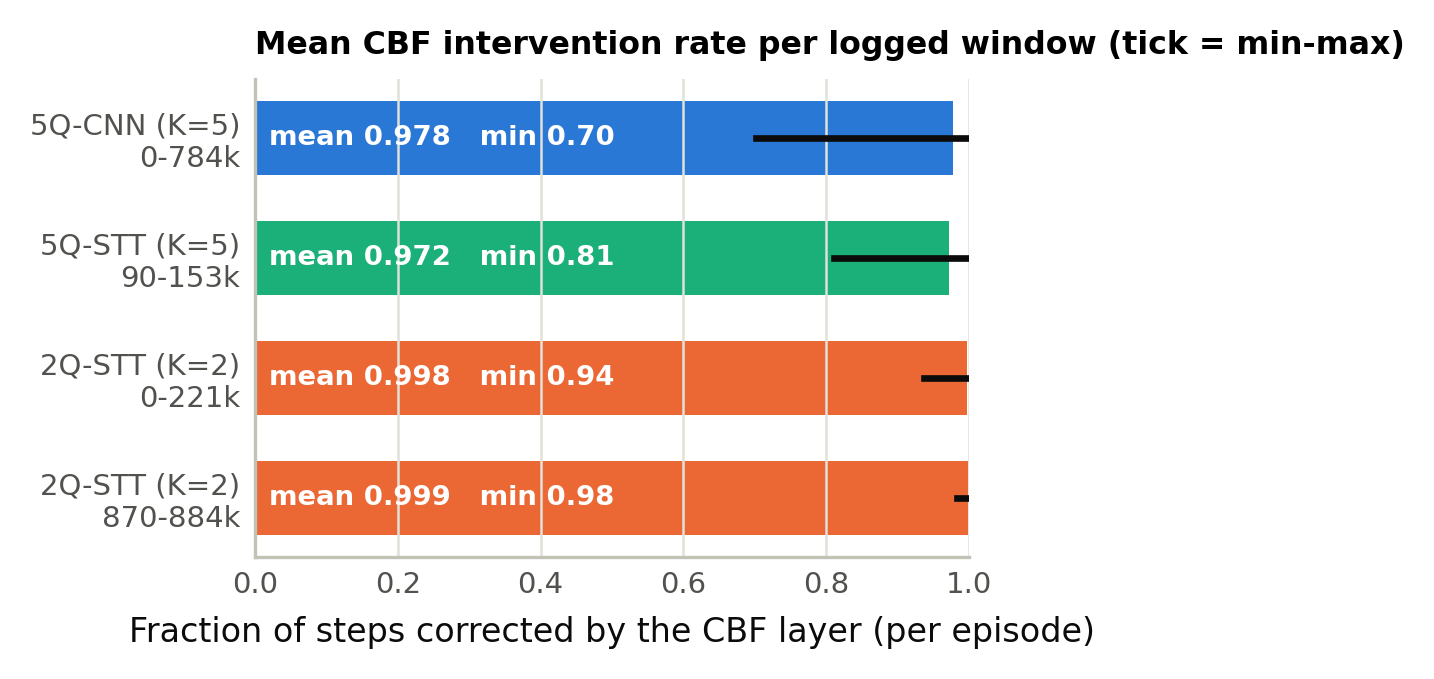
\includegraphics[width=0.95\linewidth]{Assets/cbf_invoke_rate.png}
    \caption{Mean per-episode CBF intervention rate per logged window (bar = mean, black tick = min--max). The safety layer stays engaged on the large majority of steps in every variant; the 5Q-CNN minimum of $0.70$ marks the mid-training window in which the policy's own actions transiently satisfied the barriers.}
    \label{fig:cbf}
\end{figure}

Fig.~\ref{fig:cbf} summarizes, per logged window, the fraction of steps per episode on which the QP \eqref{eq:qp} adjusted the policy's action. The layer stays engaged on the large majority of steps in every variant---mean rates of $0.978$ (5Q-CNN, full run), $0.972$ (5Q-STT), and $0.998$--$0.999$ (2Q-STT)---so the learner explores \emph{inside} a continuously active shield rather than being rescued occasionally. The full-lifetime trace also reveals structure that the partial logs concealed: the intervention rate is not flat. It dips markedly between roughly 80k and 200k steps, reaching a minimum of $0.703$, before returning to $\approx$0.98 once the agent enters the higher-speed regime visible in Fig.~\ref{fig:5qcnn}. The interpretation we favor is that the policy's actions moved transiently \emph{into} the safe set during a cautious mid-training phase, and that the shield re-engages as the agent drives faster and closer to the barriers---evidence that the correction rate is a genuine function of behavior rather than a constant artifact of over-tight constraints.

Safety outcomes under that shield are strong. Over 5Q-CNN's entire 784k-step run the mean per-episode collision rate is $0.0040$ and the mean lane-invasion rate is $0.0013$, with the final logged episodes free of both; 2Q-STT records mean collision rates of $0.007$ (early) and $0.009$ (late). The speed-limit barrier was never violated in any logged sample of any run. Mean CBF correction magnitude for 5Q-CNN is $0.245$ in action units, closing at $0.267$. On navigation, all three well-instrumented variants reached a best-episode route completion of $62.5\%$ of waypoints, though no variant completed a full route within its logged budget---which places end-to-end route completion, and the shield relaxation that should accompany it, in the future-work column rather than the results column.

\subsection{Recreating the Results}
\label{sec:recreate}
The repository ships a demo module that loads any trained checkpoint and replays the agent live in CARLA, so a reader can watch what each variant learned. With a CARLA server running,

\begin{lstlisting}[language=bash, caption={Replaying a trained agent with the demo module}, label={lst:demo}]
# 1. Start the simulator (separate terminal)
CarlaUE4.exe -fps=20 --carla-port=2000

# 2. Place a trained checkpoint where the
#    demo looks for it, e.g.:
#    demos/2stt.zip  <- sac_2q_stt_..._steps.zip

# 3. List detected models
python demo/run_model_inference.py --list-models

# 4. Watch the agent drive (N episodes)
python demo/run_model_inference.py \
    --model 2stt --episodes 3

# 5. Ablate the safety layer or the trust loop
python demo/run_model_inference.py \
    --model 2stt --episodes 3 --no-cbf
python demo/run_model_inference.py \
    --model 2stt --episodes 3 --no-trust
\end{lstlisting}

During replay the demo recomputes the trust score live from the loaded model's critic ensemble at every step---exactly as in \eqref{eq:trust}---and feeds it to the CBF layer, so the full trust-modulated safety mechanism of this paper is exercised at inference time, not only during training. The demo prints per-episode reward, waypoints crossed, collision count, the number of CBF corrections, and the episode's mean/min/max trust score, and exports the statistics to JSON for offline analysis. The \texttt{--no-cbf} flag replays the same policy without the safety layer, and \texttt{--no-trust} pins trust at 1.0, letting the reader isolate the contribution of each component directly. Training itself is equally reproducible: each experiment script accepts \texttt{--load-checkpoint} to resume from any saved zip (with its replay buffer, when present), and all figures in this section are regenerable from the TensorBoard event files with \texttt{tensorboard --logdir logs}.

\section{Discussion}
Three observations deserve emphasis. First, the trust loop---the paper's central mechanism---works as designed at the systems level: the ensemble variance is a live, state-dependent signal; it is delivered to the safety layer on schedule; and its induced trust score traverses a wide dynamic range that tracks each learner's actual convergence. Building this required touching every layer of the stack (critic architecture, training loss, callback transport, and the QP layer), and the end-to-end telemetry validates the integration.

Second, ensemble size matters more than we expected. The move from $K{=}2$ to $K{=}5$ was motivated by estimator quality, but it proved to be the difference between a converging and a non-converging critic in our setting, while the randomized $M{=}2$ min-target kept the learning targets comparable across $K$. Since the marginal cost of three extra critic MLPs is small next to CARLA simulation itself, $K{=}5$ is the configuration we recommend.

Third, the continuously engaged CBF layer reframes what ``safe training'' means in practice. Rather than the filter fading out early, our agents trained for hundreds of thousands of steps inside an active shield with low realized collision rates (mean $0.004$ per episode for 5Q-CNN across 784k steps)---exactly the operating regime one would want when the ``simulator'' is eventually a road. The non-monotone intervention rate is encouraging in this light: the dip to $0.70$ during mid-training shows the shield \emph{can} recede when the policy's own actions satisfy the barriers, which is the behavior a successful internalization would amplify. The small correction penalty and the capped trust blend \eqref{eq:blend} are the designed pathways for the policy to internalize the barriers and gradually starve the shield of work; accelerating that internalization (e.g., by annealing the penalty upward, normalizing the trust decay $\lambda$ to the evolving Q-value scale, or conditioning the policy on the route) is the clearest next step. Further future work includes equalizing training budgets across all four variants for a fully controlled $2{\times}2$ comparison, extending the occlusion protocol to the embedding-based variants, and fine-tuning the spatiotemporal encoder jointly with the policy.

\section{Limitations}
The four variants trained for unequal total step budgets (Table~\ref{tab:variants}), so whole-run comparisons should be read as characterizations of each configuration's training dynamics rather than a controlled benchmark. The central $K{=}2$ versus $K{=}5$ uncertainty comparison is an exception: it is drawn from the step-matched window 0--170k, where both configurations had received identical training budgets. Telemetry coverage is also uneven---2Q-STT and 5Q-STT have logging gaps between their early and late windows---and the reward function evolved between the earliest (2Q-CNN) run and the later ones, which is why we compare safety and uncertainty telemetry rather than raw reward across variants. Route completion was not reached within the logged budgets, and the trust decay constant $\lambda$ was fixed rather than swept. All results are from a single simulator town and a single seed per variant.

\section{Conclusion}
We presented a safety-aware DRL system for autonomous driving that closes a loop between what a learning agent knows and how tightly it is constrained: a bootstrapped critic ensemble estimates epistemic uncertainty, an exponential map turns it into a trust score, and a minimally invasive CBF-QP safety layer modulates its conservatism with that trust while shielding the agent on every step of training. Training telemetry across four system variants and $\sim$2.8M cumulative steps shows the mechanism operating exactly as intended---discriminating trust, better-calibrated uncertainty with five critics than two, and low collision rates under a continuously engaged shield---and the released code, checkpoints, and demo module let the reader reproduce both the training and the driving. We see this trust-modulated shielding pattern as a general recipe for safe learning-based control, in driving and beyond.

\bibliographystyle{IEEEtran}
\bibliography{ref}

\end{document}
